\documentclass{article}
\usepackage{graphicx} % Required for inserting images
\usepackage{graphicx}
\usepackage{fancyhdr}
\usepackage{url} % Required for inserting URLs

\pagestyle{fancy}
\fancyhf{}
\fancyhead[L]{DEIN UT4}
\fancyhead[R]{Adrian García DAM 2B}
\rfoot{\thepage}


\title{Filmosis}
\author{Proyecto Intermodular DAM, Maria Ana Sanz}
\date{Curso 2023-2024}

\begin{document}

\begin{titlepage}
    \centering

    \maketitle

    
\includegraphics[width=0.8\textwidth]{images/logo_ci_mas.jpg}

    \vspace{1cm}
    
    
\includegraphics[width=0.8\textwidth]{images/logoFilmosisPremium.png}
    
    \vspace{1cm}
    
    \textbf{Integrantes}
    
    \vspace{0.5cm}
    
    \begin{minipage}{0.5\textwidth}
        \centering
        Jiménez Aldasoro, Kaiet \\
        Arrondo Villaplana, Aritz \\
        García Galera, Adrián
    \end{minipage}
    
\end{titlepage}

\renewcommand{\contentsname}{Índice}
\tableofcontents

\newpage

\section{Introducción}

    \subsection{Breve descripción}
    
    Filmosis es una aplicación dedicada a los amantes del cine que buscan una experiencia completa para descubrir, explorar y valorar películas. Esta plataforma combina la riqueza de información de IMDb con una función de valoración integrada, permitiendo a los usuarios sumergirse en el vasto mundo del cine de una manera interactiva y social.
    
    \subsection{Objetivos}
    
        \begin{itemize}
            \item Exploración de Películas: Filmosis ofrece una amplia base de datos de películas donde los usuarios pueden explorar información detallada sobre películas, desde el elenco hasta las críticas.
            
            \item Listas Personalizadas: Los usuarios pueden crear listas personalizadas de películas, como "Mis Favoritas", "Por Ver", o cualquier categoría que deseen. Esta función ayuda a organizar y compartir preferencias cinematográficas.
            
            \item Noticias y Actualizaciones: Filmosis mantiene a los usuarios actualizados sobre las últimas noticias y eventos en la industria cinematográfica, asegurándose de que estén informados sobre estrenos, premios y más.
            
            \item Perfil de Usuario: Cada usuario tiene su propio perfil personalizado, donde pueden ver sus valoraciones, listas y contribuciones. También pueden conectarse con amigos y descubrir lo que están viendo y valorando.
        \end{itemize}
        
        Filmosis se esfuerza por crear una comunidad vibrante de cinéfilos, proporcionando una plataforma interactiva y social para explorar y disfrutar del mundo del cine.
        
        \vspace{1cm}
        
        \begin{minipage}{1\textwidth}
            \centering
            
\includegraphics[width=0.6\textwidth]{images/logoFilmosis.png}
        \end{minipage}

\section{Tecnologías empleadas}

\subsection{Kotlin}

    \begin{itemize}
        \item Retrofit: Retrofit es una biblioteca popular para Android que simplifica el consumo de servicios web RESTful. Ofrece una forma declarativa y eficiente de definir y realizar solicitudes HTTP, así como de procesar las respuestas.
    
        \item Gson: Biblioteca de Java / Kotlin desarrollada por Google que facilita el análisis y la serialización de objetos Java en formato JSON y viceversa. Es ampliamente utilizada en aplicaciones Android para el intercambio de datos entre el cliente y el servidor, así como para el almacenamiento de datos en archivos JSON.
    
        \item CarouselRecyclerView: Libearía de Android que permite crear y mostrar carruseles de elementos dentro de un RecyclerView. Esta biblioteca simplifica la implementación de carousels horizontales o verticales en aplicaciones Android, lo que proporciona una experiencia de usuario más atractiva y dinámica.
    
        \item CircleImageView: CircleImageView es una biblioteca de Android que proporciona una vista personalizada para mostrar imágenes redondeadas en aplicaciones Android. Esta biblioteca simplifica la implementación de imágenes circulares en las interfaces de usuario de las aplicaciones, lo que mejora la estética y la coherencia visual.
    
        \item Dokka: Herramienta de generación de documentación para proyectos Kotlin y Java. Esta herramienta, desarrollada por JetBrains, permite generar documentación de manera automática a partir del código fuente, facilitando la creación y mantenimiento de documentación técnica para proyectos de software.
    
        \item Glide: Glide es una biblioteca de gestión de imágenes para Android que facilita la carga, la visualización y el almacenamiento en caché de imágenes de forma eficiente en aplicaciones Android. Desarrollado por Bumptech, Glide se ha convertido en una de las bibliotecas más populares para el manejo de imágenes en el ecosistema Android.
    
    \end{itemize}

\subsection{Bibliotecas adicionales}

    \begin{itemize}
        \item Firebase: Firebase es una plataforma de desarrollo de aplicaciones móviles y web desarrollada por Google. Proporciona una variedad de servicios en la nube que ayudan a los desarrolladores a crear, mejorar y hacer crecer sus aplicaciones de manera rápida y efectiva. Estos servicios incluyen desde herramientas para el desarrollo de aplicaciones hasta análisis de usuarios y monetización. Las herramientas de Firebase que hemos utilizado son las siguientes:
    
        \begin{itemize}
            \item Firebase Analytics: Servicio de análisis de usuarios que permite a los desarrolladores comprender el comportamiento de los usuarios en sus aplicaciones, lo que les ayuda a tomar decisiones informadas para mejorar la experiencia del usuario y el rendimiento de la aplicación.
    
            \item Firebase Authentication: Servicio de autenticación de usuarios que permite a los desarrolladores autenticar usuarios de forma segura en sus aplicaciones mediante diversos métodos de autenticación, lo que garantiza la seguridad y la privacidad de los datos del usuario.
    
            \item Firebase Firestore: Firestore es un servicio de base de datos en la nube de documentos en tiempo real y escalable que permite a los desarrolladores almacenar, sincronizar y consultar datos de manera flexible y eficiente.
    
            \item Firebase Storage: Servicio de almacenamiento en la nube capaz de almacenar y servir archivos de usuario, como imágenes, videos, archivos de audio y otros archivos multimedia, de forma segura y eficiente.
        \end{itemize}
    
        \item TMDB (The Movie Database): Plataforma en línea que proporciona una amplia base de datos de información relacionada con películas, programas de televisión y personas asociadas con la industria del entretenimiento. TMDb ofrece una variedad de datos útiles para cinéfilos, desarrolladores de aplicaciones y profesionales de la industria del entretenimiento.
    \end{itemize}

\section{Estructura del proyecto}

\section{Configuración del entorno de desarrollo}

\section{Guía de Uso}
    \subsection{Instrucciones para Configurar y Ejecutar el Proyecto}

    \subsubsection{Mediante el Código Fuente (src)}

    \begin{enumerate}
        \item \textbf{Configuración inicial:}
            \begin{itemize}
                \item Abre Android Studio.
                \item Selecciona "Abrir un proyecto existente" y navega hasta el directorio donde se encuentra el código fuente del proyecto.
                \item Selecciona el archivo \texttt{build.gradle} en el directorio raíz del proyecto y haz clic en "Abrir".
            \end{itemize}
            
            \begin{figure}[h]
                \centering
                \includegraphics[width=0.8\textwidth]{Images/codigo_fuente_abrir_proyecto.png}
                \caption{Interfaz de Android Studio mostrando el proceso de apertura del proyecto existente.}
                \label{fig:codigo_fuente}
            \end{figure}
        
        \item \textbf{Espera a que Android Studio sincronice el proyecto:}
            \begin{itemize}
                \item Android Studio puede necesitar tiempo para descargar e instalar las dependencias del proyecto, así que espera a que la sincronización se complete.
            \end{itemize}
            
        \item \textbf{Configuración del dispositivo virtual o dispositivo físico:}
            \begin{itemize}
                \item Puedes ejecutar tu aplicación en un dispositivo virtual o en un dispositivo físico conectado.
                \item Para crear un dispositivo virtual, ve a \texttt{Tools > AVD Manager}, y crea un nuevo dispositivo virtual según tus preferencias.
                \item Para ejecutar en un dispositivo físico, asegúrate de tener habilitado el modo de desarrollador y la depuración USB en el dispositivo, y conéctalo a tu computadora.
            \end{itemize}
        
        \item \textbf{Ejecución del proyecto:}
            \begin{itemize}
                \item Selecciona el dispositivo en el que deseas ejecutar la aplicación (dispositivo virtual o físico) en la barra de herramientas.
                \item Haz clic en el botón "Run" (el ícono de reproducción) o presiona \texttt{Shift + F10}.
                \item Espera a que Android Studio compile el proyecto y lo ejecute en el dispositivo seleccionado.
            \end{itemize}
    \end{enumerate}

    \subsubsection{Mediante la APK Instalándola}

    \begin{enumerate}
        \item \textbf{Generación de la APK:}
            \begin{itemize}
                \item En Android Studio, ve a \texttt{Build > Build Bundle(s) / APK(s) > Build APK(s)}.
                \item Espera a que Android Studio termine de compilar el proyecto. La APK generada estará disponible en el directorio \texttt{app/build/outputs/apk/debug/}.
            \end{itemize}
            
            \begin{figure}[h]
                \centering
                \includegraphics[width=0.8\textwidth]{Images/generacion_apk_android_studio.png}
                \caption{Captura de pantalla de Android Studio durante el proceso de generación de la APK.}
                \label{fig:generacion_apk}
            \end{figure}
        
        \item \textbf{Transferencia de la APK a un Dispositivo:}
            \begin{itemize}
                \item Conecta tu dispositivo Android a tu computadora mediante un cable USB.
                \item Transfiere la APK generada al almacenamiento del dispositivo.
            \end{itemize}
        
        \item \textbf{Instalación de la APK:}
            \begin{itemize}
                \item En tu dispositivo Android, abre un explorador de archivos.
                \item Navega hasta donde hayas transferido la APK.
                \item Toca la APK para comenzar el proceso de instalación.
                \item Sigue las instrucciones en pantalla para completar la instalación.
            \end{itemize}

        \begin{figure}[h]
                \centering
                \includegraphics[width=0.3\textwidth]{Images/instalacion_apk_dispositivo.png}
                \caption{Captura de pantalla del proceso de instalación de la APK en un dispositivo Android.}
                \label{fig:instalacion_apk}
            \end{figure}
            
        \item \textbf{Ejecución de la Aplicación:}
            \begin{itemize}
                \item Una vez instalada, puedes encontrar y ejecutar la aplicación como cualquier otra aplicación en tu dispositivo Android.
            \end{itemize}
    \end{enumerate}

    \subsection{Funcionalidades principales y cómo utilizarlas}

    \subsubsection{Página de Inicio}
    % Adjuntar captura de pantalla
    La página de inicio cuenta con tres botones principales:
    \begin{itemize}
        \item \textbf{Iniciar sesión con Google:} Permite a los usuarios iniciar sesión utilizando sus cuentas de Google.
        \item \textbf{Crear una cuenta:} Permite a los nuevos usuarios crear una cuenta en la aplicación.
        \item \textbf{Iniciar sesión con usuario y contraseña:} Permite a los usuarios iniciar sesión utilizando sus credenciales de usuario.
    \end{itemize}
    Además, en la página de inicio se muestran recomendaciones de películas y películas en tendencia, junto con un buscador para encontrar películas, actores y directores.

    \subsubsection{Página de Explorar}
    % Adjuntar captura de pantalla
    En la página de explorar, los usuarios pueden:
    \begin{itemize}
        \item \textbf{Filtrar por géneros:} Se puede filtrar la lista de películas por género.
        \item \textbf{Ver películas recientes, populares, mejor valoradas y próximos estrenos:} Se muestran listas de películas organizadas por diferentes criterios.
    \end{itemize}

    \subsubsection{Perfil de Usuario}
    % Adjuntar captura de pantalla
    En el perfil de usuario, los usuarios pueden gestionar su cuenta, cambiar su foto de perfil y contraseña.

    \subsubsection{Mis Listas}
    % Adjuntar captura de pantalla
    En la sección de "Mis Listas", los usuarios pueden ver y gestionar las listas de películas que han creado.

\section{Arquitectura}

    El proyecto de Android Studio sigue una arquitectura basada en el patrón Modelo-Vista-ViewModel (MVVM) junto con elementos de la arquitectura limpia (Clean Architecture).

    \subsection{Componentes de la Arquitectura}

    \begin{itemize}
        \item \textbf{Modelo:} Las \emph{data classes} representan el Modelo en la arquitectura MVVM. Estas clases contienen los datos utilizados en la aplicación, así como la lógica relacionada con los datos.
        
        \item \textbf{Vista:} Los layouts XML definidos en el proyecto representan la Vista en la arquitectura MVVM. Estos layouts definen la estructura visual de la interfaz de usuario de la aplicación.
        
        \item \textbf{ViewModel:} Los conectores mencionados probablemente actúan como el ViewModel en la arquitectura MVVM. Estos conectores actúan como intermediarios entre la Vista y el Modelo, proporcionando los datos necesarios para la interfaz de usuario.
        
        \item \textbf{Firebase:} Se utiliza Firebase para la conexión externa, lo que implica que el proyecto también integra una capa de datos remotos. Firebase puede encajar en la arquitectura limpia como un Adaptador de Interfaces o una capa de Infraestructura, proporcionando acceso a los datos externos.
    \end{itemize}

\section{Componentes del Proyecto}

    \subsection{Layouts}

    Los layouts definidos en el proyecto definen la estructura visual de la interfaz de usuario de la aplicación. Están escritos en XML y pueden incluirse tanto en actividades como en fragmentos.

    \subsection{Activities y Fragments}

    Las actividades y fragmentos representan las diferentes pantallas y componentes de la interfaz de usuario de la aplicación.

    \subsection{Adapters}

    Los adapters se utilizan para vincular conjuntos de datos a los componentes de la interfaz de usuario, como los RecyclerViews. Estos adapters pueden proporcionar los datos necesarios desde las data classes.

    \subsection{Data Classes}

    Las data classes representan los modelos de datos utilizados en la aplicación. Contienen la información necesaria para representar los objetos en la interfaz de usuario.

    \subsection{Conectores}

    Los conectores se utilizan para interactuar con fuentes de datos externas, como Firebase. Actúan como intermediarios entre los datos externos y la lógica de la aplicación.

\section{Base de datos}

    Hemos empleado como base de datos Firestore Database, una de las opciones que nos ofrece Firebase. Firestore Database es una base de datos NoSQL, lo que significa que permite consultar datos fuera de las estructuras tradicionales que se encuentran en las bases de datos relacionales. Para almacenar los datos, hemos creado tres colecciones: Favorites, Lists y Users.
    
    \subsection{Users}
    En esta colección guardaremos los datos del inicio de sesión. Es decir, guardaremos el correo electrónico, nombre de usuario, fecha de nacimiento y, por último, nombre y apellidos.
    
    \subsection{Lists}
    En esta colección guardaremos la información de la lista. Cuando el usuario cree una lista en la base de datos, se guardará la fecha, el ID, nombre de la lista, la descripción y una lista de películas vacía. Cuando el usuario comience a añadir películas, se guardará la información de la película en la lista de películas.

\section{Documentación de código}

\section{Pruebas}

Durante el desarrollo de Filmosis, se llevaron a cabo diversas pruebas para garantizar la calidad y el funcionamiento adecuado de la aplicación. A continuación, se describen las principales pruebas realizadas:

\subsection{Pruebas Unitarias}

Las pruebas unitarias se centran en probar unidades individuales de código, como métodos o funciones, de manera aislada del resto del sistema. Estas pruebas se utilizan para verificar que cada unidad de código funcione correctamente según lo esperado. En Filmosis, se escribieron pruebas unitarias para verificar el comportamiento de funciones específicas dentro de los componentes de la aplicación, como la lógica de negocios, el manejo de datos y las interacciones con las API externas.

\subsection{Pruebas de Integración}

Las pruebas de integración evalúan la interacción entre diferentes componentes o módulos de la aplicación para asegurar que funcionen correctamente juntos. Estas pruebas son útiles para identificar problemas de comunicación o interoperabilidad entre los distintos elementos de la aplicación. En el caso de Filmosis, se realizaron pruebas de integración para verificar la comunicación adecuada entre las diferentes capas de la aplicación, como la interfaz de usuario, la lógica de negocios y el acceso a datos.

\subsection{Pruebas de Aceptación del Usuario (UAT)}

Las pruebas de aceptación del usuario implican validar la funcionalidad de la aplicación desde la perspectiva del usuario final. Estas pruebas se centran en asegurar que la aplicación cumpla con los requisitos y expectativas del usuario, así como en identificar posibles áreas de mejora desde una perspectiva de experiencia de usuario. En el caso de Filmosis, se realizaron pruebas de UAT para evaluar la usabilidad, la accesibilidad y la satisfacción general del usuario con la aplicación.

\subsection{Pruebas Unitarias en Fragmentos}

Se llevaron a cabo pruebas unitarias en los fragmentos de la aplicación para garantizar su correcto funcionamiento y comportamiento esperado. A continuación, se describen las pruebas realizadas en los fragmentos `PeliculaSeleccionadaFragment` y `ExploreFragment`:

\subsubsection{PeliculaSeleccionadaFragment}

En el fragmento `PeliculaSeleccionadaFragment`, se realizaron varias pruebas para verificar el correcto funcionamiento del cálculo del rating de la película.

\begin{itemize}
    \item \textbf{testCalculoEstrellas\_devuelve\_la\_calificación\_esperada}: Esta prueba se encarga de verificar si el cálculo del rating se realiza correctamente y devuelve la calificación esperada. Para esto, se simulan diferentes escenarios, incluyendo una calificación de cero y la calificación máxima, y se verifica si el rating calculado coincide con el rating esperado.
    
    \item \textbf{testCalculoEstrellas\_puntaje\_cero}: En esta prueba se verifica el comportamiento del cálculo del rating cuando la calificación de la película es cero. Se asegura de que el rating calculado sea igual a cero, como se espera.
    
    \item \textbf{testCalculoEstrellas\_puntaje\_maximo}: Esta prueba evalúa el cálculo del rating cuando la calificación de la película alcanza el valor máximo posible. Se verifica si el rating calculado coincide con el número máximo de estrellas, asegurando que el rating se muestre correctamente en la interfaz de usuario.
\end{itemize}

Estas pruebas aseguran que el cálculo del rating en el fragmento `PeliculaSeleccionadaFragment` funcione correctamente en una variedad de situaciones, garantizando una experiencia consistente para el usuario.

\subsubsection{ExploreFragment}

En el fragmento `ExploreFragment`, se llevaron a cabo pruebas para validar el funcionamiento de la vista de búsqueda y los botones de filtro. En la prueba `testSearchView`, se simula el ingreso de una consulta de búsqueda y se verifica que el resultado de la búsqueda sea visible en el RecyclerView correspondiente. En la prueba `testFilterButtons`, se realiza una acción de clic en un botón de filtro y se asegura que el RecyclerView de películas filtradas se actualice correctamente.

Estas pruebas unitarias en los fragmentos son fundamentales para garantizar un comportamiento consistente y sin errores en la aplicación Filmosis.






\section{Análisis de requisitos y especificaciones}

    \begin{minipage}{0.4\textwidth}
        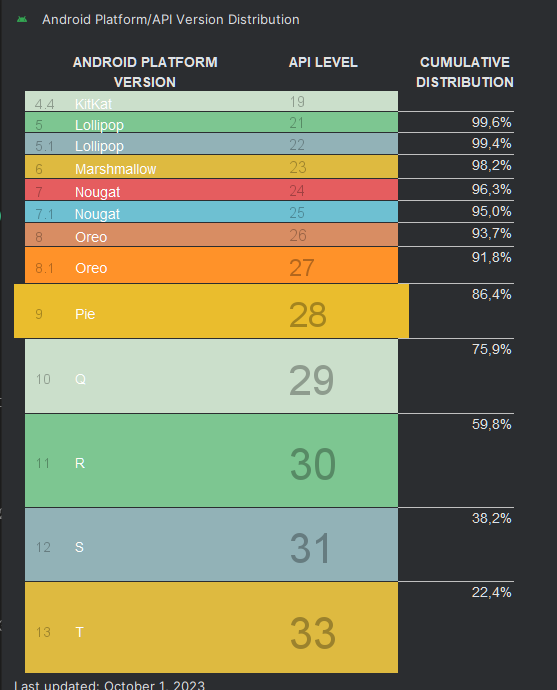
\includegraphics[width=\textwidth]{images/version.png}
    \end{minipage}
    \hfill
    \begin{minipage}{0.55\textwidth}
    Esta aplicación solo está operativa para dispositivos móviles que tengan Android como sistema operativo. Para realizar este proyecto, hemos utilizado la versión de distribución API Pie, API LEVEL 28, con una distribución acumulativa del 86.4\%. Es decir, esta aplicación solo soporta versiones con Android 9.0 como mínimo.
    \end{minipage}

\section{Consideraciones de Seguridad y Privacidad}

    En nuestro proyecto, nos tomamos muy en serio la seguridad y la privacidad de nuestros usuarios. Implementamos diversas medidas para garantizar la protección de la información confidencial y mantener la integridad de los datos. A continuación, destacamos algunas de estas consideraciones:
    
    \begin{itemize}
        \item Almacenamiento Seguro: Todos los datos sensibles se almacenan de forma segura utilizando protocolos de encriptación. Esto garantiza que la información confidencial, como contraseñas o datos personales, esté protegida contra accesos no autorizados.
    
        \item Política de Contraseñas: Aunque mencionamos que no almacenamos contraseñas, es importante destacar que fomentamos prácticas seguras de contraseñas entre nuestros usuarios. Recomendamos el uso de contraseñas únicas y complejas, así como la habilitación de la autenticación de dos factores cuando sea posible.
    
        \item Protección de Datos Personales: Cumplimos con las regulaciones de protección de datos, como el Reglamento General de Protección de Datos (GDPR), para garantizar que los datos personales de nuestros usuarios estén protegidos y se utilicen de manera ética y legal.
    
        \item Auditorías de Seguridad: Realizamos auditorías regulares de seguridad para identificar posibles vulnerabilidades en nuestro sistema y tomar medidas correctivas de manera proactiva. Esto nos ayuda a garantizar la integridad y la confidencialidad de los datos de nuestros usuarios.
    
        \item Transparencia y Comunicación: Mantenemos una comunicación abierta y transparente con nuestros usuarios sobre las medidas de seguridad y privacidad implementadas en nuestro proyecto. Esto les permite estar informados y tomar decisiones fundamentadas sobre su participación en nuestra plataforma.
        
    \end{itemize}
    
    En resumen, nuestra prioridad es garantizar la seguridad y la privacidad de nuestros usuarios en todo momento. Estamos comprometidos a seguir mejorando nuestras prácticas de seguridad y privacidad para mantener la confianza de nuestra comunidad de usuarios.

\section{Publicación y distribución}

    \subsection{Instrucciones para compilar y generar versiones de la aplicación}

    Para compilar y generar versiones de la aplicación, sigue estos pasos:
    
    \begin{enumerate}
        \item Dirígete al repositorio de GitHub de Filmosis: \url{https://github.com/agarciagale/Filmosis.git}.
        
        \item Haz clic en el botón "Code" y copia el enlace proporcionado.
        
        \item Abre tu terminal y ejecuta el siguiente comando para clonar el repositorio:
        \begin{verbatim}
            git clone <enlace_del_repositorio>
        \end{verbatim}
        
        \item Asegúrate de tener instalado un IDE compatible con Kotlin, como Android Studio.
        
        \item Navega hasta el directorio raíz del proyecto clonado en tu terminal.
        
        \item Ejecuta el siguiente comando para compilar la aplicación:
        \begin{verbatim}
            ./gradlew build
        \end{verbatim}
        Esto generará un archivo .jar en el directorio de salida del proyecto.
        
        \item Para generar una versión lista para distribuir, utiliza Gradle con el siguiente comando:
        \begin{verbatim}
            ./gradlew assembleRelease
        \end{verbatim}
        Esto generará una versión de la aplicación lista para ser distribuida.
    \end{enumerate}
    
    \subsection{Proceso de publicación en tiendas de aplicaciones o distribución interna}
    
    Para publicar la aplicación en tiendas de aplicaciones como Play Store, sigue estos pasos:
    
    \begin{enumerate}
        \item Sigue los pasos específicos de cada tienda de aplicaciones. Normalmente, necesitarás crear una cuenta de desarrollador y seguir las pautas de publicación proporcionadas por la tienda.
        
        \item Si deseas distribuir la aplicación internamente, puedes utilizar servicios como Firebase App Distribution o Google Play Console (para distribución cerrada). Configura los ajustes necesarios y sigue las instrucciones proporcionadas por el servicio elegido.
    \end{enumerate}

\section{Mantenimiento y contribuciones}

    \subsection{Políticas de Ramificación}
    
    En nuestro proyecto, hemos adoptado un enfoque de control de versiones utilizando un modelo de ramificación simple. Hemos mantenido dos ramas principales:
    
    \begin{itemize}
        \item \textbf{main}: En esta rama principal, se desarrolla el proyecto de manera activa. Aquí se encuentran las últimas características implementadas y correcciones de errores.
        
        \item \textbf{Release}: Una vez que el proyecto está listo para ser lanzado como producto, lo subimos a la rama Release. Esta rama contiene versiones estables del software que han pasado por pruebas exhaustivas y están listas para su implementación.
    \end{itemize}
    
    \subsection{Proceso de Reporte de Fallos y Gestión de Problemas}
    
    \textbf{Reporte de Fallos:}
    
    Si los usuarios encuentran algún fallo o bug, pueden reportarlo de las siguientes maneras:
    
    \begin{enumerate}
        \item \textbf{Portal de Problemas en GitHub}: Los usuarios pueden navegar al apartado de "Issues" en nuestro repositorio de GitHub. Allí, podrán ver los problemas reportados por otros usuarios y contribuir a solucionarlos si lo desean.
        
        \item \textbf{Contacto con el Equipo de Desarrollo}: Los usuarios también pueden ponerse en contacto directamente con cualquiera de los desarrolladores para informar sobre un error que hayan encontrado.
        
        \item \textbf{Pull Requests}: Si un usuario identifica un error y puede proporcionar una solución, puede enviar un "pull request" con los cambios propuestos. Esto permite una colaboración directa en la resolución de problemas.
    \end{enumerate}
    
    \textbf{Mejoras al Proceso:}
    
    Para mejorar nuestro proceso de gestión de problemas y contribuciones, estamos considerando implementar las siguientes mejoras:
    
    \begin{itemize}
        \item \textbf{Portal de Soporte Centralizado}: Estamos trabajando en la creación de un portal de soporte centralizado donde los usuarios puedan registrar sus problemas de manera estructurada, proporcionando información detallada sobre el error encontrado.
        
        \item \textbf{Formulario de Reporte de Errores}: Estamos desarrollando un formulario de reporte de errores que estandarizará la información recopilada y facilitará el seguimiento y la resolución de problemas.
        
        \item \textbf{Automatización de Gestión de Problemas}: Estamos explorando opciones para automatizar la gestión de problemas utilizando herramientas de seguimiento de problemas, lo que nos permitirá asignar responsabilidades y realizar un seguimiento más eficiente del progreso de cada problema reportado.
    \end{itemize}
    
    Estas mejoras están destinadas a hacer que nuestro proceso de reporte de fallos y gestión de problemas sea más eficiente y transparente, garantizando una mejor experiencia para nuestros usuarios y una colaboración más efectiva dentro de nuestro equipo de desarrollo.

\section{Recursos adicionales}

    \textbf{Documentación oficial de Kotlin}: \\
    \url{https://kotlinlang.org/docs/home.html} \\
    \\
    \textbf{Tutoriales en YouTube}: \\
    \url{https://youtu.be/dpURgJ4HkMk?si=k95-dp7pOh9wQ-0w} \\
    \url{https://youtu.be/jjzQvNRVhx8?si=NMKF_urWQw9Lp668} \\
    \url{https://youtu.be/vJapzH_46a8?si=2y6kzU5f11wO4W0g} \\
    \url{https://youtube.com/playlist?list=PL_QrnahGtqYAtYIoGod00kutYTvhq4HMU&si=bJn_PD4a1aPIUULR} \\
    \\
    \textbf{Comunidades y foros}: \\
    \url{https://es.stackoverflow.com/} \\
    \\
    \textbf{ChatGPT}: \\
    \url{https://chat.openai.com/}

\section{Contacto}

    Nos podéis contactar de la siguiente manera:
    \\
    \\
    Adrián García Galera: \texttt{agarciagal6@educacion.navarra.es} \\
    Aritz Arrondo Villaplana: \texttt{aarrondvil@educacion.navarra.es} \\
    Kaiet Jiménez Aldasoro: \texttt{kjimeneald@educacion.navarra.es}

\section{Conclusión}

    En resumen, Filmosis se presenta como una aplicación integral diseñada para los amantes del cine, ofreciendo una experiencia completa que combina la riqueza informativa de IMDb con características sociales interactivas. Los usuarios pueden explorar una extensa base de datos de películas, accediendo a detalles como el elenco y las críticas. La función de valoración permite a los usuarios compartir sus opiniones, descubrir películas populares y conectarse con la comunidad. La posibilidad de crear listas personalizadas facilita la organización y compartición de preferencias cinematográficas. Además, Filmosis mantiene a los usuarios informados sobre las últimas noticias y eventos en la industria cinematográfica. Con perfiles de usuario personalizados, la aplicación busca fomentar una comunidad vibrante de cinéfilos, ofreciendo una plataforma interactiva y social para explorar y disfrutar del mundo del cine.

\end{document}
